\section{Controlling the Virtual Rover}
\label{sec:control_vr_model}

In \fig\ref{fig:rover_ctrl} we depict the top-level model of the controller for the
follower vehicle. The controller is meant to operate in a loop by reading the
\emph{Velocity} of the follower rover itself, the velocity of the leader rover
(input by the \textsf{VelocityFrontObstacle} signal), the \textsf{Distance} to
the leader rover, the GPS coordinates of the leader and the rover's own GPS
coordinates.
Note that the inputs to the model appear in \fig\ref{fig:rover_ctrl}  as small
red black circles, while the outputs have the same shape but are white. By the
input values the controller constantly updates the power provided to the
wheels and it brakes when necessary. Note that the follower's and the leader's velocity are not
provided by the virtual environment -- we rather compute them outside the model
to adjust the safe distance accordingly. Although not required by the challenge,
we have implemented the computation of the speeds of the rovers to make use of
the dynamic safe distance computation provided by the original \acc model.

The controller for the virtual rover is composed by a number of \af components,
as follows:
\begin{itemize}
  \item the \textsf{TargetDistance} component is responsible for calculating the
  safe distance to the leader rover. This distance is proportional to the speed
  of the leader, as larger speeds imply larger distances for breaking. 
\item The \textsf{AngleTowardsLeader} component calculates the angle of the
follower rover towards the leader rover regarding the polar coordinates, taken
into account the GPS positions of the two rovers.
\item The \textsf{Controller} component decides which power to
provide to the wheels of the rover (separately for the left and right wheels), or whether to
apply the brakes.
\end{itemize}

\begin{figure}[!h]
\centering
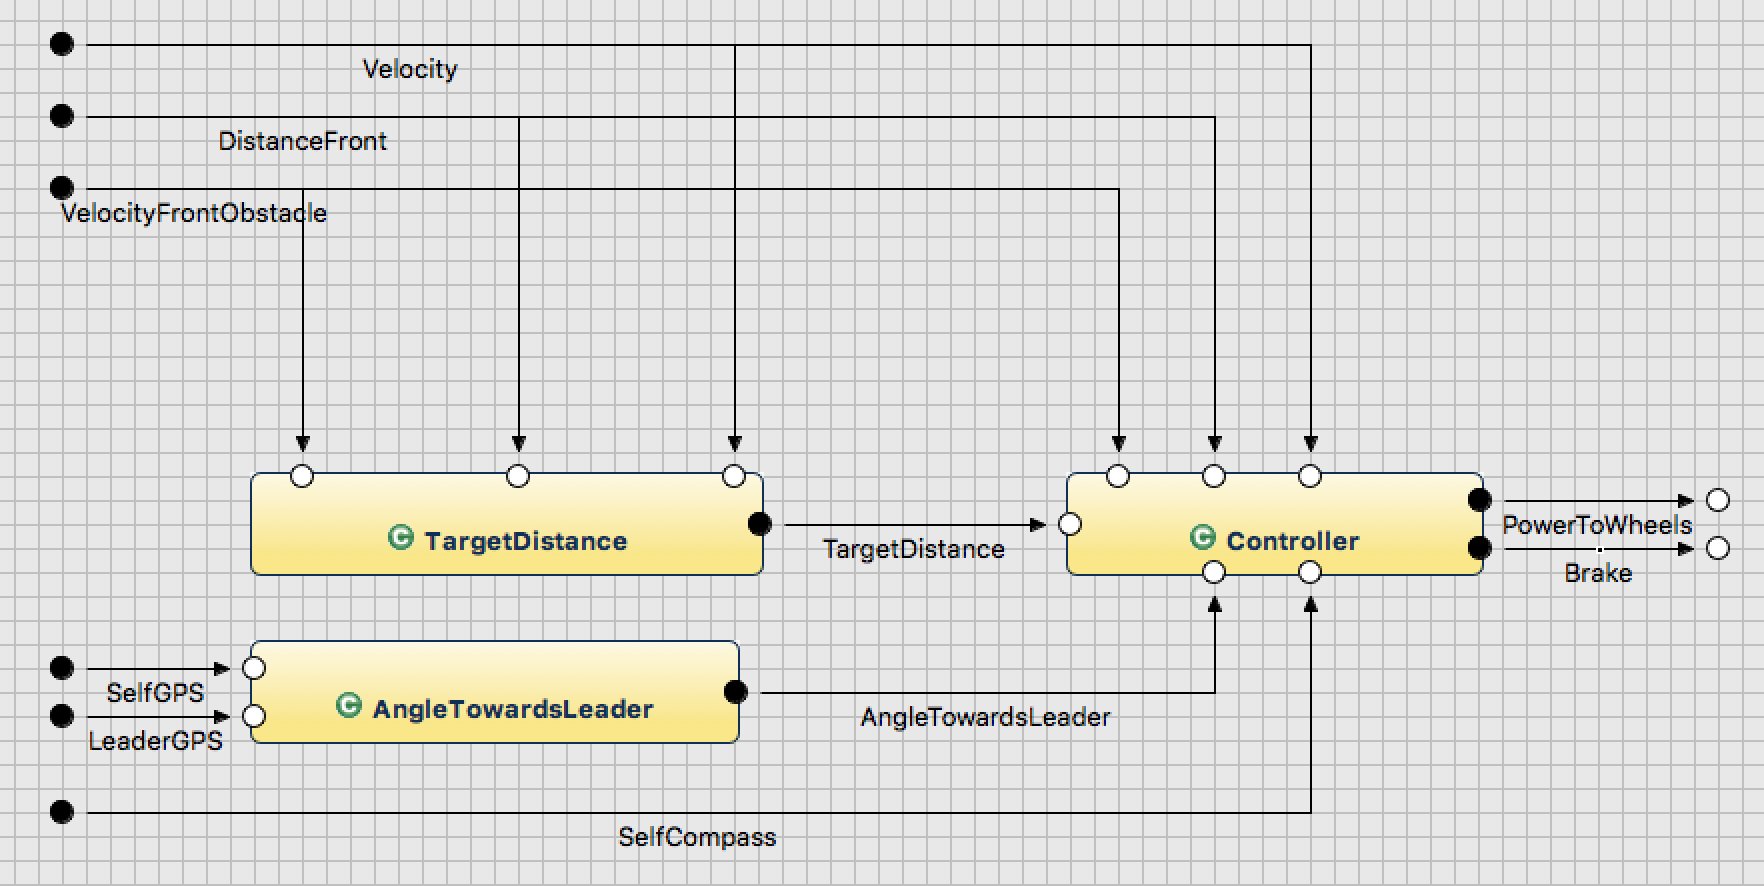
\includegraphics[width=1\textwidth]{images/top_level_controller.png}
\caption{The controller for the Virtual Rover}
\label{fig:rover_ctrl}
\end{figure}

The logic for the \emph{Controller} is partially shown in
\fig\ref{fig:controller_logic} (in the \af action language which has Java-like syntax\footnote{\af 's action
language allows for the usual imperative constructs. It is however not a
full-blown programming language as for instance variables cannot be declared
in such scripts. Such limitations were implemented in order to promote the
usage of the visual modelling part of \af, in particular of statemachines as
means to define the embedded system's state.}).
The snippet of code starts by checking whether the rover is already too close to the
leader, or the leader's speed is too low. In this case the
\textsf{TargetVelocity} is set to \textsf{0}, practically making the rover stop.

\begin{figure}[!h]
\centering
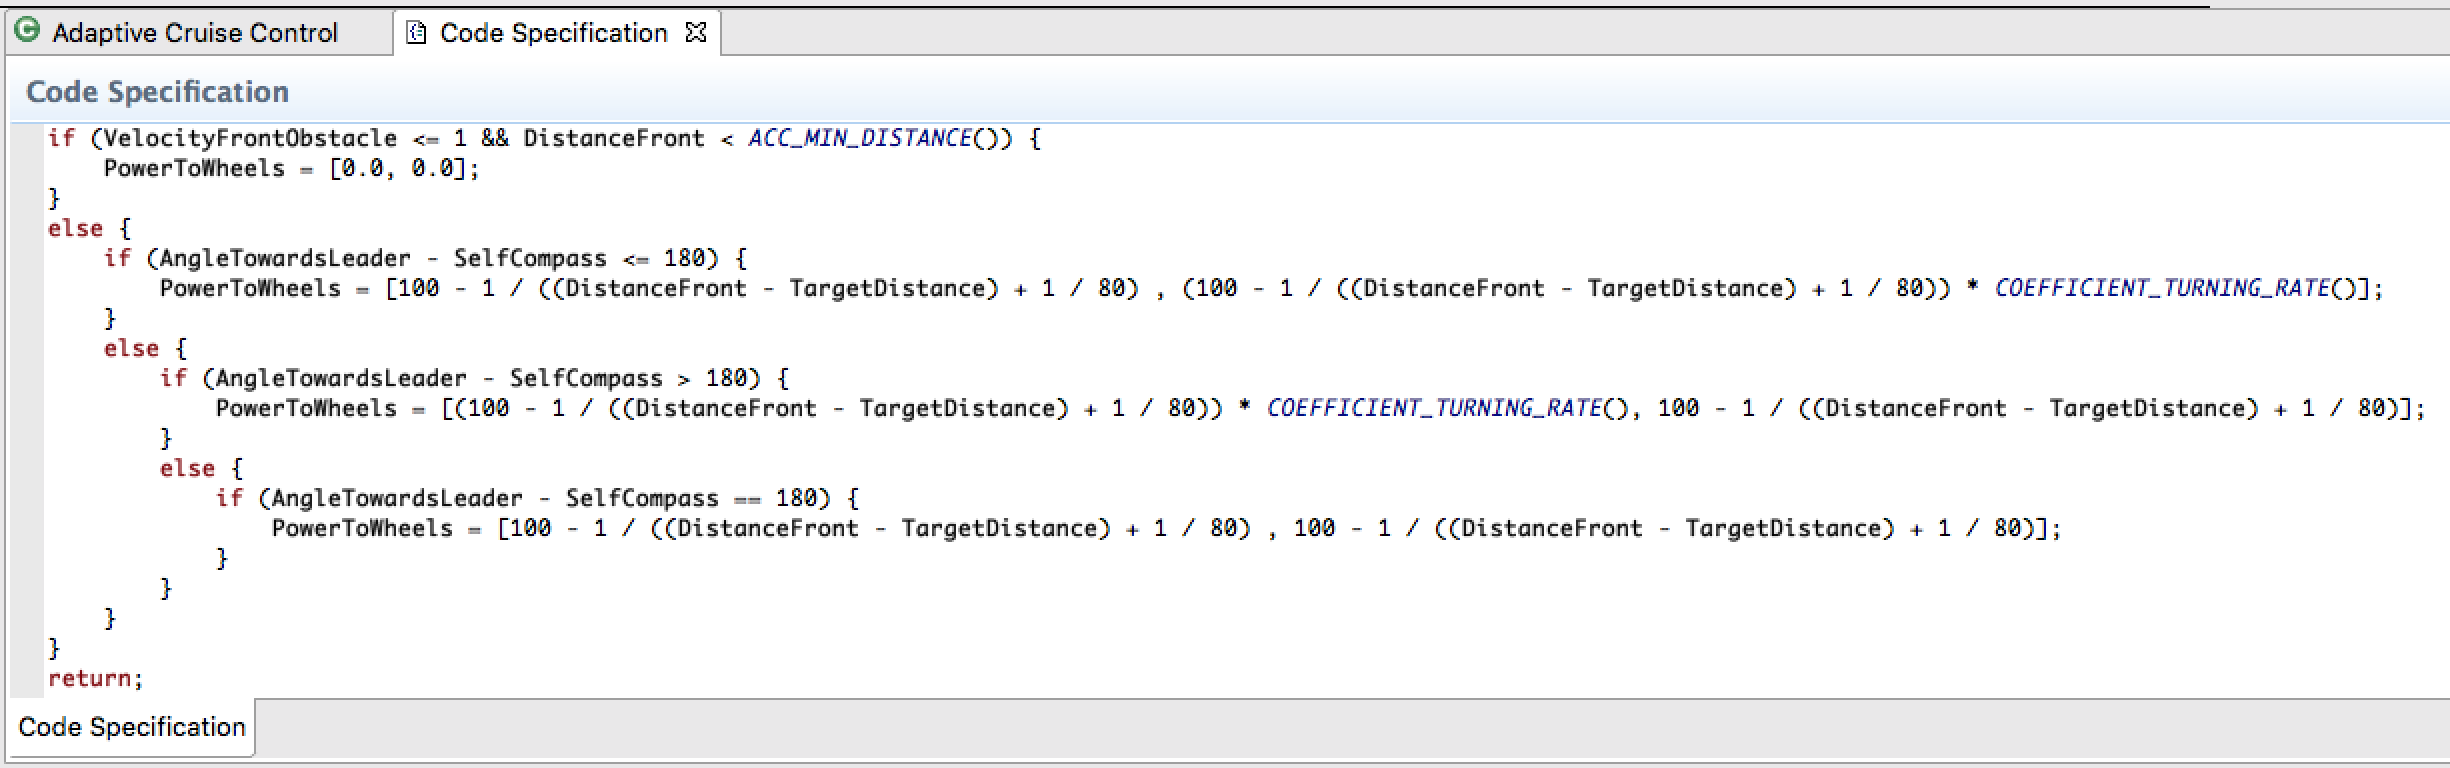
\includegraphics[width=1\textwidth]{images/code_spec_controller.png}
\caption{The Logic for the Controller Component}
\label{fig:controller_logic}
\end{figure}

The code in the snippet of code shown in \fig\ref{fig:controller_logic}
repeatedly uses formula \ref{formula:calculate_power} in order to calculate the
power to be sent to the wheels.

\begin{equation}
100 - \frac{1}{DistanceFront - TargetDistance + \frac{1}{80}}
\label{formula:calculate_power}
\end{equation}

Note that formula \ref{formula:calculate_power} tends to the value of power 20
when the \textsf{DistanceFront} and \textsf{TargetDistance} values are
very similar, or to 100 (maximum power) when the rovers are too far apart. This
translates into directing low power to the wheels when the two rovers are travelling at the
safe distance, or accelerating when the follower rover needs to catch up to the
leader. Additionally in the snippet in \fig\ref{fig:controller_logic} a
\textsf{COEFFICIENT\_TURNING\_RATE()} is multiplied by the value of the power
obtained by the formula \ref{formula:calculate_power}. The idea behind this
coefficient is that it diminishes the power directed to the left or the right
wheels, depending on where the follower rover needs to turn to in order to
follow the leader.

Note also \textsf{COEFFICIENT\_TURNING\_RATE()}  in the snippet of code in
\fig\ref{fig:controller_logic} is a function that is part of the data dictionary
of the project, partially shown in \fig\ref{fig:coefficient_turning_rate}. This function
returns the constant \textsf{0.9}. Note that functions in the data dictionary
do not only return constants and can in the general case perform complex
calculations.

\begin{figure}[!h]
\centering
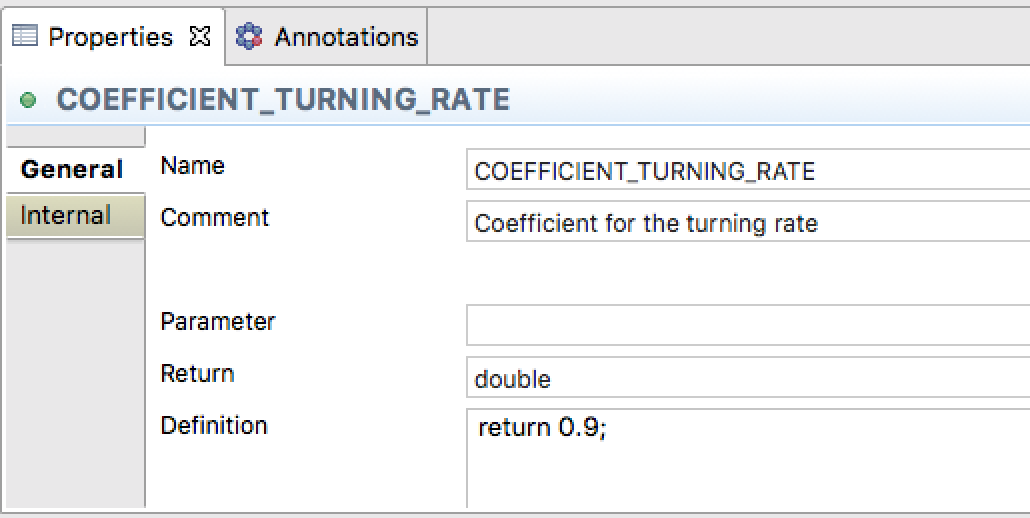
\includegraphics[width=.7\textwidth]{images/coefficient_turning_rate.png}
\caption{Coefficient for the Turning Rate} 
\label{fig:coefficient_turning_rate}
\end{figure}